%Grafo lineal
\documentclass{article}
\usepackage{tikz}
\begin{document}
\pagestyle{empty}
%Aqui se define las flechas como por defecto, mas adelante para la relacion bidireccional se definira difirente
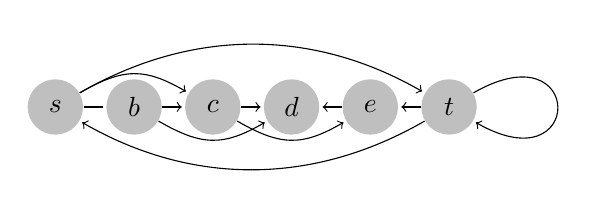
\begin{tikzpicture}[shorten >=1pt,->]
  \tikzstyle{vertex}=[circle,fill=black!25,minimum size=20pt,inner sep=0pt]

%Nodos
  \foreach \name/\x in {s/1, b/2, c/3, d/4,e/5,t/6}
    \node[vertex] (G-\name) at (\x,0) {$\name$};

%Fechas, unidireccionales 
  \foreach \from/\to in {b/c,c/d,e/d,t/e}
    \draw (G-\from) -- (G-\to);

%controls +(posicion de salida del nodo (en grados):curvatura de salida de la curva) and +(posicion de entrada del nodo (en grados):curvatura de entrada de la curva) 
%como recomendacion, la curvatura de entrada y de salida deberian sumar el numero de nodos que se van a saltar

%Algunos saltos
 \draw (G-s) .. controls +(30:2cm) and +(150:2cm) .. (G-t);
 \draw (G-s) .. controls +(30:1cm) and +(150:1cm) .. (G-c);
 \draw (G-b) .. controls +(-30:1cm) and +(-150:1cm) .. (G-d);
 \draw (G-c) .. controls +(-30:1cm) and +(-150:1cm) .. (G-e);
 \draw (G-t) .. controls +(-150:2cm) and +(-30:2cm) .. (G-s);
 \draw (G-t) .. controls +(30:2cm) and +(-30:2cm) .. (G-t);

%Relacion bidireccional
 \draw[-] (G-s) -- (G-b);

\end{tikzpicture}

\end{document}
